\documentclass[border=4pt]{standalone}
\usepackage[T1]{fontenc}
\usepackage[utf8]{inputenc}
\usepackage{lmodern}
\usepackage{tikz}
\usetikzlibrary{arrows.meta,calc}
\definecolor{azul}{HTML}{14334B}
\definecolor{acento}{HTML}{006699}
\definecolor{suave}{HTML}{EAF3F8}
\definecolor{ambar}{HTML}{94611C}
\definecolor{ftborder}{HTML}{B45309}
\definecolor{ftfill}{HTML}{FEF3C7}
\begin{document}
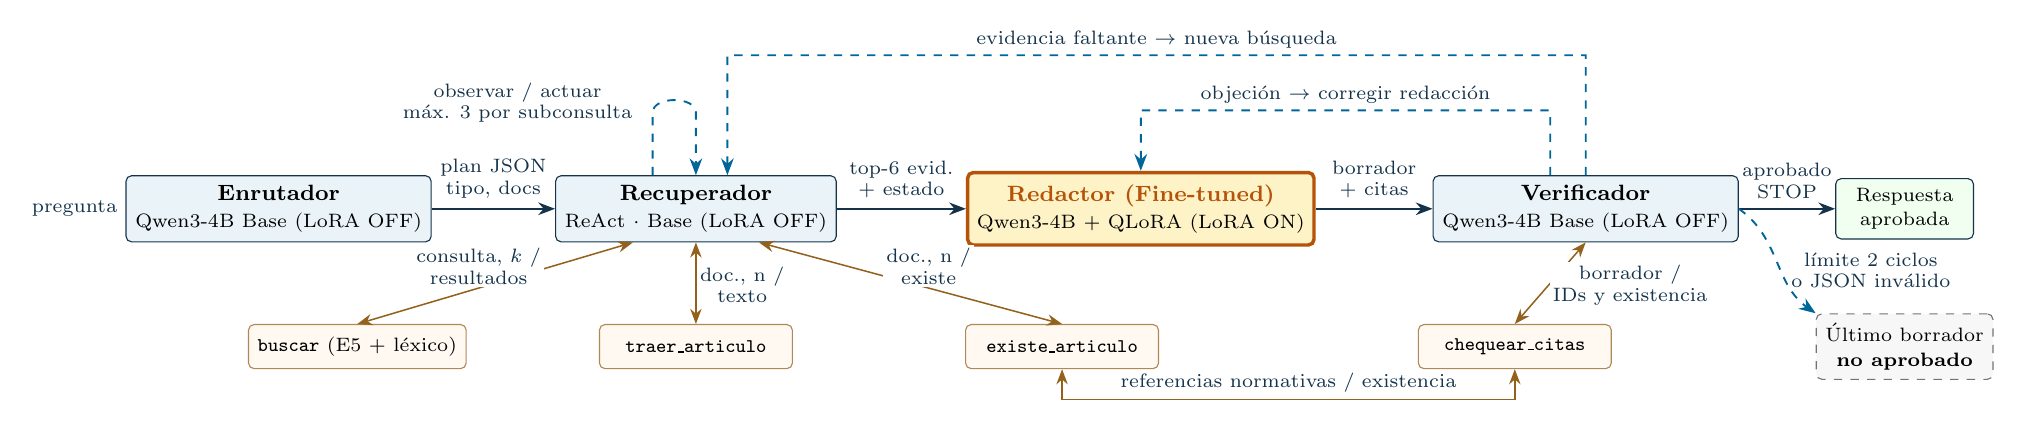
\begin{tikzpicture}[
 >=Stealth,
 agent/.style={draw=azul,fill=suave,rounded corners=2pt,minimum width=2.75cm,minimum height=0.84cm,align=center,font=\fontsize{8.5}{9.8}\selectfont},
 ftagent/.style={draw=ftborder,fill=ftfill,line width=1.25pt,rounded corners=2pt,minimum width=3.1cm,minimum height=0.92cm,align=center,font=\fontsize{8.5}{9.8}\selectfont},
 tool/.style={draw=ambar!75,fill=orange!5,rounded corners=2pt,minimum width=2.45cm,minimum height=0.56cm,align=center,font=\fontsize{7.5}{9}\selectfont},
 terminal/.style={draw=azul,fill=green!6,rounded corners=2pt,minimum width=1.75cm,minimum height=0.74cm,align=center,font=\fontsize{7.5}{9}\selectfont},
 lab/.style={fill=white,inner sep=1.2pt,align=center,font=\fontsize{6.8}{7.8}\selectfont,text=azul},
 flab/.style={inner sep=1.5pt,align=center,font=\fontsize{6.8}{7.8}\selectfont,text=azul},
 flow/.style={->,draw=azul,line width=0.68pt},
 back/.style={->,draw=acento,dashed,line width=0.68pt},
 use/.style={<->,draw=ambar,line width=0.55pt}
]
\node[agent] (e) at (1.40,0) {\textbf{Enrutador}\\{\fontsize{6.8}{7.8}\selectfont Qwen3-4B Base (LoRA OFF)}};
\node[agent] (r) at (6.70,0) {\textbf{Recuperador}\\{\fontsize{6.8}{7.8}\selectfont ReAct $\cdot$ Base (LoRA OFF)}};
\node[ftagent] (w) at (12.35,0) {{\color{ftborder}\textbf{Redactor (Fine-tuned)}}\\{\fontsize{6.8}{7.8}\selectfont Qwen3-4B + QLoRA (LoRA ON)}};
\node[agent] (v) at (18.00,0) {\textbf{Verificador}\\{\fontsize{6.8}{7.8}\selectfont Qwen3-4B Base (LoRA OFF)}};
\node[terminal] (out) at (22.05,0) {Respuesta\\aprobada};
\node[terminal,fill=black!3,draw=black!55,dashed] (stop) at (22.05,-1.75) {Último borrador\\\textbf{no aprobado}};

\draw[flow] (e.east)--node[flab,above=2pt]{plan JSON\\tipo, docs}(r.west);
\draw[flow] (r.east)--node[flab,above=2pt]{top-6 evid.\\+ estado}(w.west);
\draw[flow] (w.east)--node[flab,above=2pt]{borrador\\+ citas}(v.west);
\draw[flow] (v.east)--node[flab,above=2pt]{aprobado\\STOP}(out.west);
\draw[back] (v.east) to[out=-35,in=145] node[lab,pos=.58,right=2pt,font=\fontsize{6.8}{7.8}\selectfont]{límite 2 ciclos\\o JSON inválido}(stop.north west);
\node[flab,anchor=east] at (e.west) {pregunta\,};

\draw[back] ($(v.north)+(-.45,0)$) -- (17.55,1.25) -- node[lab,above=1pt,pos=.5]{objeción $\rightarrow$ corregir redacción} (12.35,1.25) -- (w.north);
\draw[back] (v.north) -- (18.00,1.95) -- node[lab,above=1pt]{evidencia faltante $\rightarrow$ nueva búsqueda} (7.10,1.95) -- ($(r.north)+(.4,0)$);
\draw[back] ($(r.north)+(-.55,0)$) -- (6.15,1.22) to[out=90,in=90] (6.70,1.22) -- ($(r.north)+(0,0)$);
\node[flab,anchor=east] at (5.95,1.35) {observar / actuar\\máx. 3 por subconsulta};

\node[tool] (b) at (2.40,-1.75) {\texttt{buscar} (E5 + léxico)};
\node[tool] (a) at (6.70,-1.75) {\texttt{traer\_articulo}};
\node[tool] (x) at (11.35,-1.75) {\texttt{existe\_articulo}};
\node[tool] (c) at (17.10,-1.75) {\texttt{chequear\_citas}};
\draw[use] ($(r.south)+(-.8,0)$)--node[lab,pos=.56,above]{consulta, $k$ /\\resultados}(b.north);
\draw[use] (r.south)--node[lab,right,pos=.52]{doc., n /\\texto}(a.north);
\draw[use] ($(r.south)+(.8,0)$)--node[lab,pos=.56,above]{doc., n /\\existe}(x.north);
\draw[use] (v.south)--node[lab,right,pos=.52]{borrador /\\IDs y existencia}(c.north);
\draw[use] (c.south)--(17.10,-2.42)--node[lab,above=1pt]{referencias normativas / existencia}(11.35,-2.42)--(x.south);
\end{tikzpicture}
\end{document}
